% Created by tikzDevice version 0.10.1 on 2018-02-17 17:12:12
% !TEX encoding = UTF-8 Unicode
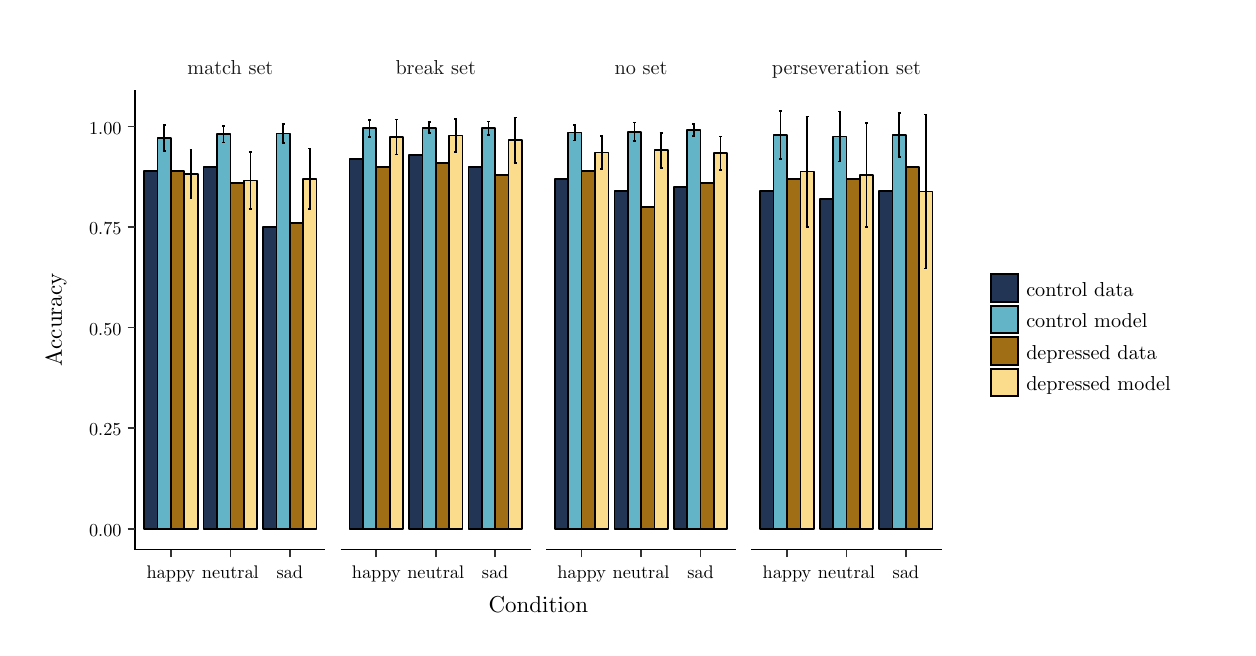
\begin{tikzpicture}[x=1pt,y=1pt]
\definecolor{fillColor}{RGB}{255,255,255}
\path[use as bounding box,fill=fillColor,fill opacity=0.00] (0,0) rectangle (433.62,216.81);
\begin{scope}
\path[clip] (  0.00,  0.00) rectangle (433.62,216.81);
\definecolor{drawColor}{RGB}{255,255,255}
\definecolor{fillColor}{RGB}{255,255,255}

\path[draw=drawColor,line width= 0.6pt,line join=round,line cap=round,fill=fillColor] (  0.00,  0.00) rectangle (433.62,216.81);
\end{scope}
\begin{scope}
\path[clip] ( 38.88, 28.22) rectangle (107.59,194.25);
\definecolor{fillColor}{RGB}{255,255,255}

\path[fill=fillColor] ( 38.88, 28.22) rectangle (107.59,194.25);
\definecolor{drawColor}{RGB}{0,0,0}
\definecolor{fillColor}{RGB}{250,220,140}

\path[draw=drawColor,line width= 0.6pt,line join=round,fill=fillColor] ( 56.60, 35.77) rectangle ( 61.43,163.94);
\definecolor{fillColor}{RGB}{160,110,20}

\path[draw=drawColor,line width= 0.6pt,line join=round,fill=fillColor] ( 51.77, 35.77) rectangle ( 56.60,165.09);
\definecolor{fillColor}{RGB}{100,180,200}

\path[draw=drawColor,line width= 0.6pt,line join=round,fill=fillColor] ( 46.94, 35.77) rectangle ( 51.77,176.97);
\definecolor{fillColor}{RGB}{35,53,85}

\path[draw=drawColor,line width= 0.6pt,line join=round,fill=fillColor] ( 42.11, 35.77) rectangle ( 46.94,165.09);
\definecolor{fillColor}{RGB}{250,220,140}

\path[draw=drawColor,line width= 0.6pt,line join=round,fill=fillColor] ( 78.07, 35.77) rectangle ( 82.90,161.63);
\definecolor{fillColor}{RGB}{160,110,20}

\path[draw=drawColor,line width= 0.6pt,line join=round,fill=fillColor] ( 73.24, 35.77) rectangle ( 78.07,160.73);
\definecolor{fillColor}{RGB}{100,180,200}

\path[draw=drawColor,line width= 0.6pt,line join=round,fill=fillColor] ( 68.41, 35.77) rectangle ( 73.24,178.33);
\definecolor{fillColor}{RGB}{35,53,85}

\path[draw=drawColor,line width= 0.6pt,line join=round,fill=fillColor] ( 63.58, 35.77) rectangle ( 68.41,166.54);
\definecolor{fillColor}{RGB}{250,220,140}

\path[draw=drawColor,line width= 0.6pt,line join=round,fill=fillColor] ( 99.54, 35.77) rectangle (104.37,162.17);
\definecolor{fillColor}{RGB}{160,110,20}

\path[draw=drawColor,line width= 0.6pt,line join=round,fill=fillColor] ( 94.71, 35.77) rectangle ( 99.54,146.20);
\definecolor{fillColor}{RGB}{100,180,200}

\path[draw=drawColor,line width= 0.6pt,line join=round,fill=fillColor] ( 89.88, 35.77) rectangle ( 94.71,178.58);
\definecolor{fillColor}{RGB}{35,53,85}

\path[draw=drawColor,line width= 0.6pt,line join=round,fill=fillColor] ( 85.05, 35.77) rectangle ( 89.88,144.75);

\path[draw=drawColor,line width= 0.6pt,line join=round] ( 58.48,172.84) --
	( 59.55,172.84);

\path[draw=drawColor,line width= 0.6pt,line join=round] ( 59.01,172.84) --
	( 59.01,155.03);

\path[draw=drawColor,line width= 0.6pt,line join=round] ( 58.48,155.03) --
	( 59.55,155.03);

\path[draw=drawColor,line width= 0.6pt,line join=round] ( 48.81,181.66) --
	( 49.89,181.66);

\path[draw=drawColor,line width= 0.6pt,line join=round] ( 49.35,181.66) --
	( 49.35,172.27);

\path[draw=drawColor,line width= 0.6pt,line join=round] ( 48.81,172.27) --
	( 49.89,172.27);

\path[draw=drawColor,line width= 0.6pt,line join=round] ( 79.95,172.00) --
	( 81.02,172.00);

\path[draw=drawColor,line width= 0.6pt,line join=round] ( 80.49,172.00) --
	( 80.49,151.26);

\path[draw=drawColor,line width= 0.6pt,line join=round] ( 79.95,151.26) --
	( 81.02,151.26);

\path[draw=drawColor,line width= 0.6pt,line join=round] ( 70.29,181.37) --
	( 71.36,181.37);

\path[draw=drawColor,line width= 0.6pt,line join=round] ( 70.82,181.37) --
	( 70.82,175.29);

\path[draw=drawColor,line width= 0.6pt,line join=round] ( 70.29,175.29) --
	( 71.36,175.29);

\path[draw=drawColor,line width= 0.6pt,line join=round] (101.42,173.17) --
	(102.49,173.17);

\path[draw=drawColor,line width= 0.6pt,line join=round] (101.96,173.17) --
	(101.96,151.18);

\path[draw=drawColor,line width= 0.6pt,line join=round] (101.42,151.18) --
	(102.49,151.18);

\path[draw=drawColor,line width= 0.6pt,line join=round] ( 91.76,181.96) --
	( 92.83,181.96);

\path[draw=drawColor,line width= 0.6pt,line join=round] ( 92.29,181.96) --
	( 92.29,175.21);

\path[draw=drawColor,line width= 0.6pt,line join=round] ( 91.76,175.21) --
	( 92.83,175.21);
\end{scope}
\begin{scope}
\path[clip] (113.09, 28.22) rectangle (181.80,194.25);
\definecolor{fillColor}{RGB}{255,255,255}

\path[fill=fillColor] (113.09, 28.22) rectangle (181.80,194.25);
\definecolor{drawColor}{RGB}{0,0,0}
\definecolor{fillColor}{RGB}{250,220,140}

\path[draw=drawColor,line width= 0.6pt,line join=round,fill=fillColor] (130.81, 35.77) rectangle (135.64,177.25);
\definecolor{fillColor}{RGB}{160,110,20}

\path[draw=drawColor,line width= 0.6pt,line join=round,fill=fillColor] (125.98, 35.77) rectangle (130.81,166.54);
\definecolor{fillColor}{RGB}{100,180,200}

\path[draw=drawColor,line width= 0.6pt,line join=round,fill=fillColor] (121.14, 35.77) rectangle (125.98,180.48);
\definecolor{fillColor}{RGB}{35,53,85}

\path[draw=drawColor,line width= 0.6pt,line join=round,fill=fillColor] (116.31, 35.77) rectangle (121.14,169.45);
\definecolor{fillColor}{RGB}{250,220,140}

\path[draw=drawColor,line width= 0.6pt,line join=round,fill=fillColor] (152.28, 35.77) rectangle (157.11,177.82);
\definecolor{fillColor}{RGB}{160,110,20}

\path[draw=drawColor,line width= 0.6pt,line join=round,fill=fillColor] (147.45, 35.77) rectangle (152.28,168.00);
\definecolor{fillColor}{RGB}{100,180,200}

\path[draw=drawColor,line width= 0.6pt,line join=round,fill=fillColor] (142.62, 35.77) rectangle (147.45,180.67);
\definecolor{fillColor}{RGB}{35,53,85}

\path[draw=drawColor,line width= 0.6pt,line join=round,fill=fillColor] (137.78, 35.77) rectangle (142.62,170.90);
\definecolor{fillColor}{RGB}{250,220,140}

\path[draw=drawColor,line width= 0.6pt,line join=round,fill=fillColor] (173.75, 35.77) rectangle (178.58,176.15);
\definecolor{fillColor}{RGB}{160,110,20}

\path[draw=drawColor,line width= 0.6pt,line join=round,fill=fillColor] (168.92, 35.77) rectangle (173.75,163.64);
\definecolor{fillColor}{RGB}{100,180,200}

\path[draw=drawColor,line width= 0.6pt,line join=round,fill=fillColor] (164.09, 35.77) rectangle (168.92,180.48);
\definecolor{fillColor}{RGB}{35,53,85}

\path[draw=drawColor,line width= 0.6pt,line join=round,fill=fillColor] (159.26, 35.77) rectangle (164.09,166.54);

\path[draw=drawColor,line width= 0.6pt,line join=round] (132.69,183.59) --
	(133.76,183.59);

\path[draw=drawColor,line width= 0.6pt,line join=round] (133.22,183.59) --
	(133.22,170.92);

\path[draw=drawColor,line width= 0.6pt,line join=round] (132.69,170.92) --
	(133.76,170.92);

\path[draw=drawColor,line width= 0.6pt,line join=round] (123.02,183.56) --
	(124.10,183.56);

\path[draw=drawColor,line width= 0.6pt,line join=round] (123.56,183.56) --
	(123.56,177.40);

\path[draw=drawColor,line width= 0.6pt,line join=round] (123.02,177.40) --
	(124.10,177.40);

\path[draw=drawColor,line width= 0.6pt,line join=round] (154.16,183.86) --
	(155.23,183.86);

\path[draw=drawColor,line width= 0.6pt,line join=round] (154.69,183.86) --
	(154.69,171.78);

\path[draw=drawColor,line width= 0.6pt,line join=round] (154.16,171.78) --
	(155.23,171.78);

\path[draw=drawColor,line width= 0.6pt,line join=round] (144.49,182.68) --
	(145.57,182.68);

\path[draw=drawColor,line width= 0.6pt,line join=round] (145.03,182.68) --
	(145.03,178.65);

\path[draw=drawColor,line width= 0.6pt,line join=round] (144.49,178.65) --
	(145.57,178.65);

\path[draw=drawColor,line width= 0.6pt,line join=round] (175.63,184.39) --
	(176.70,184.39);

\path[draw=drawColor,line width= 0.6pt,line join=round] (176.16,184.39) --
	(176.16,167.90);

\path[draw=drawColor,line width= 0.6pt,line join=round] (175.63,167.90) --
	(176.70,167.90);

\path[draw=drawColor,line width= 0.6pt,line join=round] (165.97,182.87) --
	(167.04,182.87);

\path[draw=drawColor,line width= 0.6pt,line join=round] (166.50,182.87) --
	(166.50,178.09);

\path[draw=drawColor,line width= 0.6pt,line join=round] (165.97,178.09) --
	(167.04,178.09);
\end{scope}
\begin{scope}
\path[clip] (187.30, 28.22) rectangle (256.01,194.25);
\definecolor{fillColor}{RGB}{255,255,255}

\path[fill=fillColor] (187.30, 28.22) rectangle (256.01,194.25);
\definecolor{drawColor}{RGB}{0,0,0}
\definecolor{fillColor}{RGB}{250,220,140}

\path[draw=drawColor,line width= 0.6pt,line join=round,fill=fillColor] (205.01, 35.77) rectangle (209.85,171.74);
\definecolor{fillColor}{RGB}{160,110,20}

\path[draw=drawColor,line width= 0.6pt,line join=round,fill=fillColor] (200.18, 35.77) rectangle (205.01,165.09);
\definecolor{fillColor}{RGB}{100,180,200}

\path[draw=drawColor,line width= 0.6pt,line join=round,fill=fillColor] (195.35, 35.77) rectangle (200.18,178.87);
\definecolor{fillColor}{RGB}{35,53,85}

\path[draw=drawColor,line width= 0.6pt,line join=round,fill=fillColor] (190.52, 35.77) rectangle (195.35,162.18);
\definecolor{fillColor}{RGB}{250,220,140}

\path[draw=drawColor,line width= 0.6pt,line join=round,fill=fillColor] (226.49, 35.77) rectangle (231.32,172.52);
\definecolor{fillColor}{RGB}{160,110,20}

\path[draw=drawColor,line width= 0.6pt,line join=round,fill=fillColor] (221.65, 35.77) rectangle (226.49,152.01);
\definecolor{fillColor}{RGB}{100,180,200}

\path[draw=drawColor,line width= 0.6pt,line join=round,fill=fillColor] (216.82, 35.77) rectangle (221.65,179.21);
\definecolor{fillColor}{RGB}{35,53,85}

\path[draw=drawColor,line width= 0.6pt,line join=round,fill=fillColor] (211.99, 35.77) rectangle (216.82,157.83);
\definecolor{fillColor}{RGB}{250,220,140}

\path[draw=drawColor,line width= 0.6pt,line join=round,fill=fillColor] (247.96, 35.77) rectangle (252.79,171.50);
\definecolor{fillColor}{RGB}{160,110,20}

\path[draw=drawColor,line width= 0.6pt,line join=round,fill=fillColor] (243.13, 35.77) rectangle (247.96,160.73);
\definecolor{fillColor}{RGB}{100,180,200}

\path[draw=drawColor,line width= 0.6pt,line join=round,fill=fillColor] (238.29, 35.77) rectangle (243.13,179.86);
\definecolor{fillColor}{RGB}{35,53,85}

\path[draw=drawColor,line width= 0.6pt,line join=round,fill=fillColor] (233.46, 35.77) rectangle (238.29,159.28);

\path[draw=drawColor,line width= 0.6pt,line join=round] (206.89,177.68) --
	(207.97,177.68);

\path[draw=drawColor,line width= 0.6pt,line join=round] (207.43,177.68) --
	(207.43,165.80);

\path[draw=drawColor,line width= 0.6pt,line join=round] (206.89,165.80) --
	(207.97,165.80);

\path[draw=drawColor,line width= 0.6pt,line join=round] (197.23,181.69) --
	(198.30,181.69);

\path[draw=drawColor,line width= 0.6pt,line join=round] (197.77,181.69) --
	(197.77,176.05);

\path[draw=drawColor,line width= 0.6pt,line join=round] (197.23,176.05) --
	(198.30,176.05);

\path[draw=drawColor,line width= 0.6pt,line join=round] (228.36,178.82) --
	(229.44,178.82);

\path[draw=drawColor,line width= 0.6pt,line join=round] (228.90,178.82) --
	(228.90,166.21);

\path[draw=drawColor,line width= 0.6pt,line join=round] (228.36,166.21) --
	(229.44,166.21);

\path[draw=drawColor,line width= 0.6pt,line join=round] (218.70,182.51) --
	(219.78,182.51);

\path[draw=drawColor,line width= 0.6pt,line join=round] (219.24,182.51) --
	(219.24,175.91);

\path[draw=drawColor,line width= 0.6pt,line join=round] (218.70,175.91) --
	(219.78,175.91);

\path[draw=drawColor,line width= 0.6pt,line join=round] (249.84,177.52) --
	(250.91,177.52);

\path[draw=drawColor,line width= 0.6pt,line join=round] (250.37,177.52) --
	(250.37,165.48);

\path[draw=drawColor,line width= 0.6pt,line join=round] (249.84,165.48) --
	(250.91,165.48);

\path[draw=drawColor,line width= 0.6pt,line join=round] (240.17,181.94) --
	(241.25,181.94);

\path[draw=drawColor,line width= 0.6pt,line join=round] (240.71,181.94) --
	(240.71,177.78);

\path[draw=drawColor,line width= 0.6pt,line join=round] (240.17,177.78) --
	(241.25,177.78);
\end{scope}
\begin{scope}
\path[clip] (261.51, 28.22) rectangle (330.22,194.25);
\definecolor{fillColor}{RGB}{255,255,255}

\path[fill=fillColor] (261.51, 28.22) rectangle (330.22,194.25);
\definecolor{drawColor}{RGB}{0,0,0}
\definecolor{fillColor}{RGB}{250,220,140}

\path[draw=drawColor,line width= 0.6pt,line join=round,fill=fillColor] (279.22, 35.77) rectangle (284.05,164.79);
\definecolor{fillColor}{RGB}{160,110,20}

\path[draw=drawColor,line width= 0.6pt,line join=round,fill=fillColor] (274.39, 35.77) rectangle (279.22,162.18);
\definecolor{fillColor}{RGB}{100,180,200}

\path[draw=drawColor,line width= 0.6pt,line join=round,fill=fillColor] (269.56, 35.77) rectangle (274.39,178.07);
\definecolor{fillColor}{RGB}{35,53,85}

\path[draw=drawColor,line width= 0.6pt,line join=round,fill=fillColor] (264.73, 35.77) rectangle (269.56,157.83);
\definecolor{fillColor}{RGB}{250,220,140}

\path[draw=drawColor,line width= 0.6pt,line join=round,fill=fillColor] (300.69, 35.77) rectangle (305.52,163.53);
\definecolor{fillColor}{RGB}{160,110,20}

\path[draw=drawColor,line width= 0.6pt,line join=round,fill=fillColor] (295.86, 35.77) rectangle (300.69,162.18);
\definecolor{fillColor}{RGB}{100,180,200}

\path[draw=drawColor,line width= 0.6pt,line join=round,fill=fillColor] (291.03, 35.77) rectangle (295.86,177.54);
\definecolor{fillColor}{RGB}{35,53,85}

\path[draw=drawColor,line width= 0.6pt,line join=round,fill=fillColor] (286.20, 35.77) rectangle (291.03,154.92);
\definecolor{fillColor}{RGB}{250,220,140}

\path[draw=drawColor,line width= 0.6pt,line join=round,fill=fillColor] (322.16, 35.77) rectangle (327.00,157.59);
\definecolor{fillColor}{RGB}{160,110,20}

\path[draw=drawColor,line width= 0.6pt,line join=round,fill=fillColor] (317.33, 35.77) rectangle (322.16,166.54);
\definecolor{fillColor}{RGB}{100,180,200}

\path[draw=drawColor,line width= 0.6pt,line join=round,fill=fillColor] (312.50, 35.77) rectangle (317.33,177.99);
\definecolor{fillColor}{RGB}{35,53,85}

\path[draw=drawColor,line width= 0.6pt,line join=round,fill=fillColor] (307.67, 35.77) rectangle (312.50,157.83);

\path[draw=drawColor,line width= 0.6pt,line join=round] (281.10,184.75) --
	(282.17,184.75);

\path[draw=drawColor,line width= 0.6pt,line join=round] (281.64,184.75) --
	(281.64,144.82);

\path[draw=drawColor,line width= 0.6pt,line join=round] (281.10,144.82) --
	(282.17,144.82);

\path[draw=drawColor,line width= 0.6pt,line join=round] (271.44,186.70) --
	(272.51,186.70);

\path[draw=drawColor,line width= 0.6pt,line join=round] (271.98,186.70) --
	(271.98,169.44);

\path[draw=drawColor,line width= 0.6pt,line join=round] (271.44,169.44) --
	(272.51,169.44);

\path[draw=drawColor,line width= 0.6pt,line join=round] (302.57,182.29) --
	(303.65,182.29);

\path[draw=drawColor,line width= 0.6pt,line join=round] (303.11,182.29) --
	(303.11,144.78);

\path[draw=drawColor,line width= 0.6pt,line join=round] (302.57,144.78) --
	(303.65,144.78);

\path[draw=drawColor,line width= 0.6pt,line join=round] (292.91,186.57) --
	(293.98,186.57);

\path[draw=drawColor,line width= 0.6pt,line join=round] (293.45,186.57) --
	(293.45,168.51);

\path[draw=drawColor,line width= 0.6pt,line join=round] (292.91,168.51) --
	(293.98,168.51);

\path[draw=drawColor,line width= 0.6pt,line join=round] (324.04,185.43) --
	(325.12,185.43);

\path[draw=drawColor,line width= 0.6pt,line join=round] (324.58,185.43) --
	(324.58,129.74);

\path[draw=drawColor,line width= 0.6pt,line join=round] (324.04,129.74) --
	(325.12,129.74);

\path[draw=drawColor,line width= 0.6pt,line join=round] (314.38,185.95) --
	(315.46,185.95);

\path[draw=drawColor,line width= 0.6pt,line join=round] (314.92,185.95) --
	(314.92,170.04);

\path[draw=drawColor,line width= 0.6pt,line join=round] (314.38,170.04) --
	(315.46,170.04);
\end{scope}
\begin{scope}
\path[clip] ( 38.88,194.25) rectangle (107.59,211.31);
\definecolor{drawColor}{RGB}{255,255,255}
\definecolor{fillColor}{RGB}{255,255,255}

\path[draw=drawColor,line width= 1.1pt,line join=round,line cap=round,fill=fillColor] ( 38.88,194.25) rectangle (107.59,211.31);
\definecolor{drawColor}{gray}{0.10}

\node[text=drawColor,anchor=base,inner sep=0pt, outer sep=0pt, scale=  0.73] at ( 73.24,199.75) {match set};
\end{scope}
\begin{scope}
\path[clip] (113.09,194.25) rectangle (181.80,211.31);
\definecolor{drawColor}{RGB}{255,255,255}
\definecolor{fillColor}{RGB}{255,255,255}

\path[draw=drawColor,line width= 1.1pt,line join=round,line cap=round,fill=fillColor] (113.09,194.25) rectangle (181.80,211.31);
\definecolor{drawColor}{gray}{0.10}

\node[text=drawColor,anchor=base,inner sep=0pt, outer sep=0pt, scale=  0.73] at (147.45,199.75) {break set};
\end{scope}
\begin{scope}
\path[clip] (187.30,194.25) rectangle (256.01,211.31);
\definecolor{drawColor}{RGB}{255,255,255}
\definecolor{fillColor}{RGB}{255,255,255}

\path[draw=drawColor,line width= 1.1pt,line join=round,line cap=round,fill=fillColor] (187.30,194.25) rectangle (256.01,211.31);
\definecolor{drawColor}{gray}{0.10}

\node[text=drawColor,anchor=base,inner sep=0pt, outer sep=0pt, scale=  0.73] at (221.65,199.75) {no set};
\end{scope}
\begin{scope}
\path[clip] (261.51,194.25) rectangle (330.22,211.31);
\definecolor{drawColor}{RGB}{255,255,255}
\definecolor{fillColor}{RGB}{255,255,255}

\path[draw=drawColor,line width= 1.1pt,line join=round,line cap=round,fill=fillColor] (261.51,194.25) rectangle (330.22,211.31);
\definecolor{drawColor}{gray}{0.10}

\node[text=drawColor,anchor=base,inner sep=0pt, outer sep=0pt, scale=  0.73] at (295.86,199.75) {perseveration set};
\end{scope}
\begin{scope}
\path[clip] (  0.00,  0.00) rectangle (433.62,216.81);
\definecolor{drawColor}{RGB}{0,0,0}

\path[draw=drawColor,line width= 0.6pt,line join=round] ( 38.88, 28.22) --
	(107.59, 28.22);
\end{scope}
\begin{scope}
\path[clip] (  0.00,  0.00) rectangle (433.62,216.81);
\definecolor{drawColor}{gray}{0.20}

\path[draw=drawColor,line width= 0.6pt,line join=round] ( 51.77, 25.47) --
	( 51.77, 28.22);

\path[draw=drawColor,line width= 0.6pt,line join=round] ( 73.24, 25.47) --
	( 73.24, 28.22);

\path[draw=drawColor,line width= 0.6pt,line join=round] ( 94.71, 25.47) --
	( 94.71, 28.22);
\end{scope}
\begin{scope}
\path[clip] (  0.00,  0.00) rectangle (433.62,216.81);
\definecolor{drawColor}{RGB}{0,0,0}

\node[text=drawColor,anchor=base,inner sep=0pt, outer sep=0pt, scale=  0.66] at ( 51.77, 17.82) {happy};

\node[text=drawColor,anchor=base,inner sep=0pt, outer sep=0pt, scale=  0.66] at ( 73.24, 17.82) {neutral};

\node[text=drawColor,anchor=base,inner sep=0pt, outer sep=0pt, scale=  0.66] at ( 94.71, 17.82) {sad};
\end{scope}
\begin{scope}
\path[clip] (  0.00,  0.00) rectangle (433.62,216.81);
\definecolor{drawColor}{RGB}{0,0,0}

\path[draw=drawColor,line width= 0.6pt,line join=round] (113.09, 28.22) --
	(181.80, 28.22);
\end{scope}
\begin{scope}
\path[clip] (  0.00,  0.00) rectangle (433.62,216.81);
\definecolor{drawColor}{gray}{0.20}

\path[draw=drawColor,line width= 0.6pt,line join=round] (125.98, 25.47) --
	(125.98, 28.22);

\path[draw=drawColor,line width= 0.6pt,line join=round] (147.45, 25.47) --
	(147.45, 28.22);

\path[draw=drawColor,line width= 0.6pt,line join=round] (168.92, 25.47) --
	(168.92, 28.22);
\end{scope}
\begin{scope}
\path[clip] (  0.00,  0.00) rectangle (433.62,216.81);
\definecolor{drawColor}{RGB}{0,0,0}

\node[text=drawColor,anchor=base,inner sep=0pt, outer sep=0pt, scale=  0.66] at (125.98, 17.82) {happy};

\node[text=drawColor,anchor=base,inner sep=0pt, outer sep=0pt, scale=  0.66] at (147.45, 17.82) {neutral};

\node[text=drawColor,anchor=base,inner sep=0pt, outer sep=0pt, scale=  0.66] at (168.92, 17.82) {sad};
\end{scope}
\begin{scope}
\path[clip] (  0.00,  0.00) rectangle (433.62,216.81);
\definecolor{drawColor}{RGB}{0,0,0}

\path[draw=drawColor,line width= 0.6pt,line join=round] (187.30, 28.22) --
	(256.01, 28.22);
\end{scope}
\begin{scope}
\path[clip] (  0.00,  0.00) rectangle (433.62,216.81);
\definecolor{drawColor}{gray}{0.20}

\path[draw=drawColor,line width= 0.6pt,line join=round] (200.18, 25.47) --
	(200.18, 28.22);

\path[draw=drawColor,line width= 0.6pt,line join=round] (221.65, 25.47) --
	(221.65, 28.22);

\path[draw=drawColor,line width= 0.6pt,line join=round] (243.13, 25.47) --
	(243.13, 28.22);
\end{scope}
\begin{scope}
\path[clip] (  0.00,  0.00) rectangle (433.62,216.81);
\definecolor{drawColor}{RGB}{0,0,0}

\node[text=drawColor,anchor=base,inner sep=0pt, outer sep=0pt, scale=  0.66] at (200.18, 17.82) {happy};

\node[text=drawColor,anchor=base,inner sep=0pt, outer sep=0pt, scale=  0.66] at (221.65, 17.82) {neutral};

\node[text=drawColor,anchor=base,inner sep=0pt, outer sep=0pt, scale=  0.66] at (243.13, 17.82) {sad};
\end{scope}
\begin{scope}
\path[clip] (  0.00,  0.00) rectangle (433.62,216.81);
\definecolor{drawColor}{RGB}{0,0,0}

\path[draw=drawColor,line width= 0.6pt,line join=round] (261.51, 28.22) --
	(330.22, 28.22);
\end{scope}
\begin{scope}
\path[clip] (  0.00,  0.00) rectangle (433.62,216.81);
\definecolor{drawColor}{gray}{0.20}

\path[draw=drawColor,line width= 0.6pt,line join=round] (274.39, 25.47) --
	(274.39, 28.22);

\path[draw=drawColor,line width= 0.6pt,line join=round] (295.86, 25.47) --
	(295.86, 28.22);

\path[draw=drawColor,line width= 0.6pt,line join=round] (317.33, 25.47) --
	(317.33, 28.22);
\end{scope}
\begin{scope}
\path[clip] (  0.00,  0.00) rectangle (433.62,216.81);
\definecolor{drawColor}{RGB}{0,0,0}

\node[text=drawColor,anchor=base,inner sep=0pt, outer sep=0pt, scale=  0.66] at (274.39, 17.82) {happy};

\node[text=drawColor,anchor=base,inner sep=0pt, outer sep=0pt, scale=  0.66] at (295.86, 17.82) {neutral};

\node[text=drawColor,anchor=base,inner sep=0pt, outer sep=0pt, scale=  0.66] at (317.33, 17.82) {sad};
\end{scope}
\begin{scope}
\path[clip] (  0.00,  0.00) rectangle (433.62,216.81);
\definecolor{drawColor}{RGB}{0,0,0}

\path[draw=drawColor,line width= 0.6pt,line join=round] ( 38.88, 28.22) --
	( 38.88,194.25);
\end{scope}
\begin{scope}
\path[clip] (  0.00,  0.00) rectangle (433.62,216.81);
\definecolor{drawColor}{RGB}{0,0,0}

\node[text=drawColor,anchor=base east,inner sep=0pt, outer sep=0pt, scale=  0.66] at ( 33.93, 33.04) {0.00};

\node[text=drawColor,anchor=base east,inner sep=0pt, outer sep=0pt, scale=  0.66] at ( 33.93, 69.37) {0.25};

\node[text=drawColor,anchor=base east,inner sep=0pt, outer sep=0pt, scale=  0.66] at ( 33.93,105.69) {0.50};

\node[text=drawColor,anchor=base east,inner sep=0pt, outer sep=0pt, scale=  0.66] at ( 33.93,142.02) {0.75};

\node[text=drawColor,anchor=base east,inner sep=0pt, outer sep=0pt, scale=  0.66] at ( 33.93,178.35) {1.00};
\end{scope}
\begin{scope}
\path[clip] (  0.00,  0.00) rectangle (433.62,216.81);
\definecolor{drawColor}{gray}{0.20}

\path[draw=drawColor,line width= 0.6pt,line join=round] ( 36.13, 35.77) --
	( 38.88, 35.77);

\path[draw=drawColor,line width= 0.6pt,line join=round] ( 36.13, 72.10) --
	( 38.88, 72.10);

\path[draw=drawColor,line width= 0.6pt,line join=round] ( 36.13,108.42) --
	( 38.88,108.42);

\path[draw=drawColor,line width= 0.6pt,line join=round] ( 36.13,144.75) --
	( 38.88,144.75);

\path[draw=drawColor,line width= 0.6pt,line join=round] ( 36.13,181.07) --
	( 38.88,181.07);
\end{scope}
\begin{scope}
\path[clip] (  0.00,  0.00) rectangle (433.62,216.81);
\definecolor{drawColor}{RGB}{0,0,0}

\node[text=drawColor,anchor=base,inner sep=0pt, outer sep=0pt, scale=  0.83] at (184.55,  5.50) {Condition};
\end{scope}
\begin{scope}
\path[clip] (  0.00,  0.00) rectangle (433.62,216.81);
\definecolor{drawColor}{RGB}{0,0,0}

\node[text=drawColor,rotate= 90.00,anchor=base,inner sep=0pt, outer sep=0pt, scale=  0.83] at ( 12.32,111.24) {Accuracy};
\end{scope}
\begin{scope}
\path[clip] (  0.00,  0.00) rectangle (433.62,216.81);
\definecolor{fillColor}{RGB}{255,255,255}

\path[fill=fillColor] (341.60, 77.21) rectangle (428.12,145.27);
\end{scope}
\begin{scope}
\path[clip] (  0.00,  0.00) rectangle (433.62,216.81);
\definecolor{drawColor}{RGB}{0,0,0}
\definecolor{fillColor}{RGB}{35,53,85}

\path[draw=drawColor,line width= 0.6pt,line cap=round,fill=fillColor] (348.00,117.75) rectangle (357.96,127.71);
\end{scope}
\begin{scope}
\path[clip] (  0.00,  0.00) rectangle (433.62,216.81);
\definecolor{drawColor}{RGB}{0,0,0}
\definecolor{fillColor}{RGB}{100,180,200}

\path[draw=drawColor,line width= 0.6pt,line cap=round,fill=fillColor] (348.00,106.37) rectangle (357.96,116.33);
\end{scope}
\begin{scope}
\path[clip] (  0.00,  0.00) rectangle (433.62,216.81);
\definecolor{drawColor}{RGB}{0,0,0}
\definecolor{fillColor}{RGB}{160,110,20}

\path[draw=drawColor,line width= 0.6pt,line cap=round,fill=fillColor] (348.00, 94.99) rectangle (357.96,104.95);
\end{scope}
\begin{scope}
\path[clip] (  0.00,  0.00) rectangle (433.62,216.81);
\definecolor{drawColor}{RGB}{0,0,0}
\definecolor{fillColor}{RGB}{250,220,140}

\path[draw=drawColor,line width= 0.6pt,line cap=round,fill=fillColor] (348.00, 83.61) rectangle (357.96, 93.57);
\end{scope}
\begin{scope}
\path[clip] (  0.00,  0.00) rectangle (433.62,216.81);
\definecolor{drawColor}{RGB}{0,0,0}

\node[text=drawColor,anchor=base west,inner sep=0pt, outer sep=0pt, scale=  0.73] at (360.84,119.70) {control data};
\end{scope}
\begin{scope}
\path[clip] (  0.00,  0.00) rectangle (433.62,216.81);
\definecolor{drawColor}{RGB}{0,0,0}

\node[text=drawColor,anchor=base west,inner sep=0pt, outer sep=0pt, scale=  0.73] at (360.84,108.32) {control model};
\end{scope}
\begin{scope}
\path[clip] (  0.00,  0.00) rectangle (433.62,216.81);
\definecolor{drawColor}{RGB}{0,0,0}

\node[text=drawColor,anchor=base west,inner sep=0pt, outer sep=0pt, scale=  0.73] at (360.84, 96.94) {depressed data};
\end{scope}
\begin{scope}
\path[clip] (  0.00,  0.00) rectangle (433.62,216.81);
\definecolor{drawColor}{RGB}{0,0,0}

\node[text=drawColor,anchor=base west,inner sep=0pt, outer sep=0pt, scale=  0.73] at (360.84, 85.56) {depressed model};
\end{scope}
\end{tikzpicture}
